\documentclass[tikz,border=8pt]{standalone}
\usepackage{amsmath}
\usepackage{pgfplots}
\pgfplotsset{compat=1.18}
\usepgfplotslibrary{groupplots}
\usetikzlibrary{calc}
\definecolor{ink}{HTML}{21352F}
\definecolor{teal}{HTML}{087F7B}
\definecolor{gold}{HTML}{C58B2A}
\definecolor{blue}{HTML}{4B77A8}
\definecolor{rose}{HTML}{B65A62}
\begin{document}
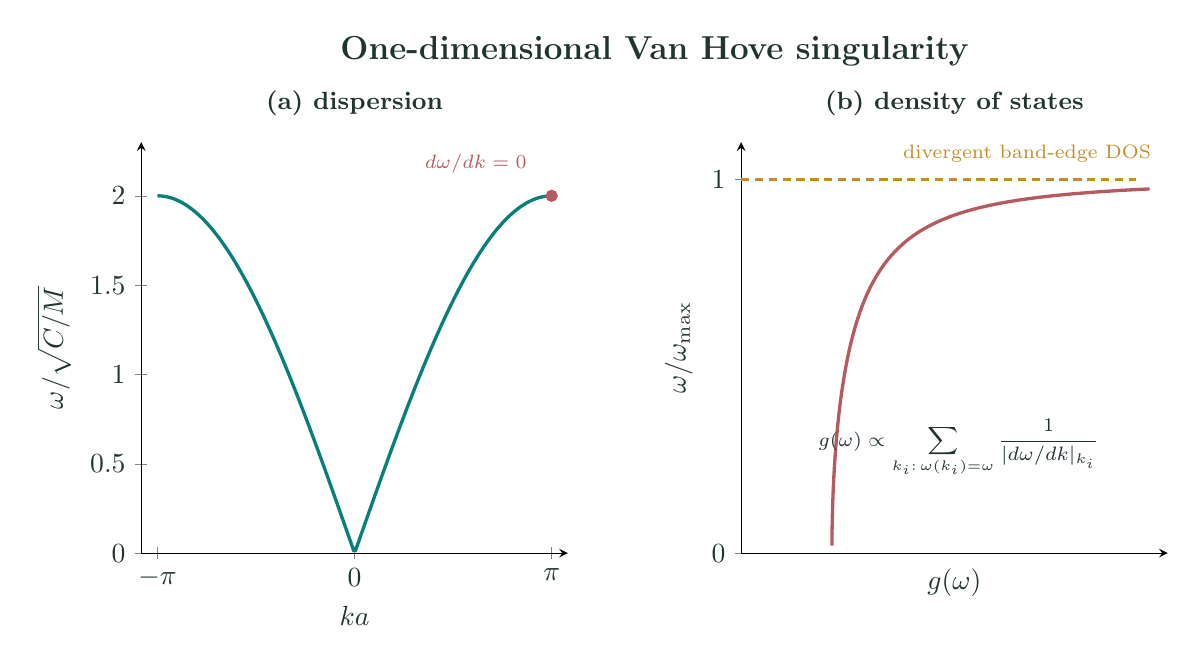
\begin{tikzpicture}[font=\sffamily,text=ink]
  \begin{groupplot}[
    group style={group size=2 by 1,horizontal sep=2.2cm},
    width=7.0cm,height=6.8cm,
    axis lines=left]
  \nextgroupplot[
    xmin=-3.4,xmax=3.4,ymin=0,ymax=2.3,
    xlabel={$ka$},ylabel={$\omega/\sqrt{C/M}$},
    xtick={-3.14159,0,3.14159},xticklabels={$-\pi$,$0$,$\pi$},
    title={(a) dispersion},title style={font=\bfseries\small}]
    \addplot[teal,very thick,domain=-3.14159:3.14159,samples=220]
      {2*abs(sin(deg(x)/2))};
    \draw[rose,fill=rose] (axis cs:3.14159,2) circle (2pt);
    \node[rose,font=\scriptsize,anchor=east] at (axis cs:2.9,2.18) {$d\omega/dk=0$};
  \nextgroupplot[
    xmin=0,xmax=4.7,ymin=0,ymax=1.1,
    xlabel={$g(\omega)$},ylabel={$\omega/\omega_{\max}$},
    xtick=\empty,ytick={0,1},yticklabels={$0$,$1$},
    title={(b) density of states},title style={font=\bfseries\small},clip=false]
    \addplot[rose,very thick,domain=.02:.975,samples=220,variable=\y]
      ({1/sqrt(1-\y^2)},\y);
    \draw[gold,densely dashed,thick] (axis cs:0,1)--(axis cs:4.35,1);
    \node[gold,font=\scriptsize,anchor=south] at (axis cs:3.15,1.02) {divergent band-edge DOS};
    \node[font=\scriptsize,align=center] at (axis cs:2.4,.28)
      {$\displaystyle g(\omega)\propto
        \sum_{k_i:\,\omega(k_i)=\omega}
        \frac{1}{\lvert d\omega/dk\rvert_{k_i}}$};
  \end{groupplot}
  \node[font=\bfseries\large] at ($(group c1r1.north)!0.5!(group c2r1.north)+(0,1.15)$)
    {One-dimensional Van Hove singularity};
\end{tikzpicture}
\end{document}
